\chapter[Elements of Nuclear Physics]{Elements of Nuclear Physics}\label{chap3}

\Authorline{V Devanathan\footnote[*]{Email: \url{vdevanathan@hotmail.com}}}

\authinfo{
The Academy of Sciences, Chennai\\
Department of Nuclear Physics\\
University of Madras, Guindy Campus\\
Chennai - 600 025}

\begin{abstract}
The study of Nuclear Physics can be broadly classified into two parts; the static part and the dynamic part. The static part consists of the study of nuclear energy levels, their binding energies, the magnetic dipole moments and the electric quadrupole moments. The dynamic part deals with the transition of nuclei from one energy level to another due to interactions with external agencies including elementary particles. The former involves the evaluation of matrix elements with spherical tensor operators and the latter the calculation of transition probability from one nuclear state to another. This article briefly outlines how the transition probability can be calculated and how the method can be applied to the study of photoproduction of pions from nuclei. This was an emerging field, about sixty years ago, and this article presents some initial attempts made by G. Ramachandram and I to study this problem.
\end{abstract}

\section{Introduction}\label{chap3-sec1}
 
It was with Professor G. Ramachandran that I started to learn the elements of Nuclear Physics in the late Nineteen fifties when we commenced our research career \cite{chap3-key1,chap3-key2,chap3-key3,chap3-key4,chap3-key5,chap3-key6,chap3-key7,chap3-key8} under the guidance of Prof.\ Alladi Ramakrishnan, in the University of Madras. Earlier, Prof.\ Alladi had done remarkable work in the field of Stochastic Processes using the concept of Product Densities, known now as Ramakrishnan Product Densities. In the year 1958, he spent a year at the Institute for Advanced Studies at Princeton which had an exhilarating influence on him and his interest shifted from Stochastic Processes to Elementary Particles and Nuclear Physics. It had also brought about a great change in his vision and motivated him to create such a centre in India. On his return to India, he started one-year M.Sc.\ Course in Theoretical Physics which attracted a large number of brilliant students to join the course. Soon, he was promoted as Professor and posted to the newly started extension centre at Madurai but permitted to run the M.Sc.\ Program, already started, in Madras. It was a nebulous situation. Since Prof.\ Alladi had a palatial ancestral home - Ekamra Nivas, he conducted most of the classes in the spacious hall on the first floor of his house. Since Elementary particles and Nuclear Physics were new areas of study, everyone was encouraged to give lectures on different topics. The learning process may truly be called a boot-strap mechanism.

The informal group was given the name “Theoretical Physics Seminar” and we started inviting the visiting scientists from abroad to give talks at the Seminar. Visit to Mahabalipuram and dinner at New Woodlands were the usual way of extending the hospitality to the visiting scientists. A.M. Lane, Abdus Salam, Donald Glaser, S. Chandrasekhar were some of the distinguished scientists who gave talks at the Seminar. A few of them stayed as in-house guests of Prof.\ Alladi. They are scientists of high calibre. Donald Glaser already received the Nobel Prize for his invention of Bubble Chamber and Abdus Salam and S. Chandrasekhar received the Nobel Prizes subsequently. Abdus Salam was responsible for setting up the International Centre for Theoretical Physics at Trieste, which offered the opportunity for young scientists from developing countries to participate in its research activities as visiting scientists. Photographs of the Theoretical Physics Seminar Group taken with Abdus Salam, Donald Glaser and S. Chandrasekhar are attached herewith.

It was a fortunate coincidence that both Niels Bohr and Abdus Salam visited Madras in January 1960, after attending the Indian Science\break Congress held at Bombay and the Theoretical Physics Seminar hosted a dinner in honour of both in New Woodlands. Niels Bohr was very much impressed by the efforts of Alladi in gathering a small enthusiastic group of young theoretical physicists and communicated the same to the then Prime Minister of India, Jawaharlal Nehru, which ultimately resulted in the establishment of the Institute of Mathematical Sciences at Madras 	on January 3, 1962 on the pattern of Institute for Advanced Studies at Princeton \cite{chap3-key9}.
\medskip

%~ \begin{figure}[H]
%~ \centering
%~ 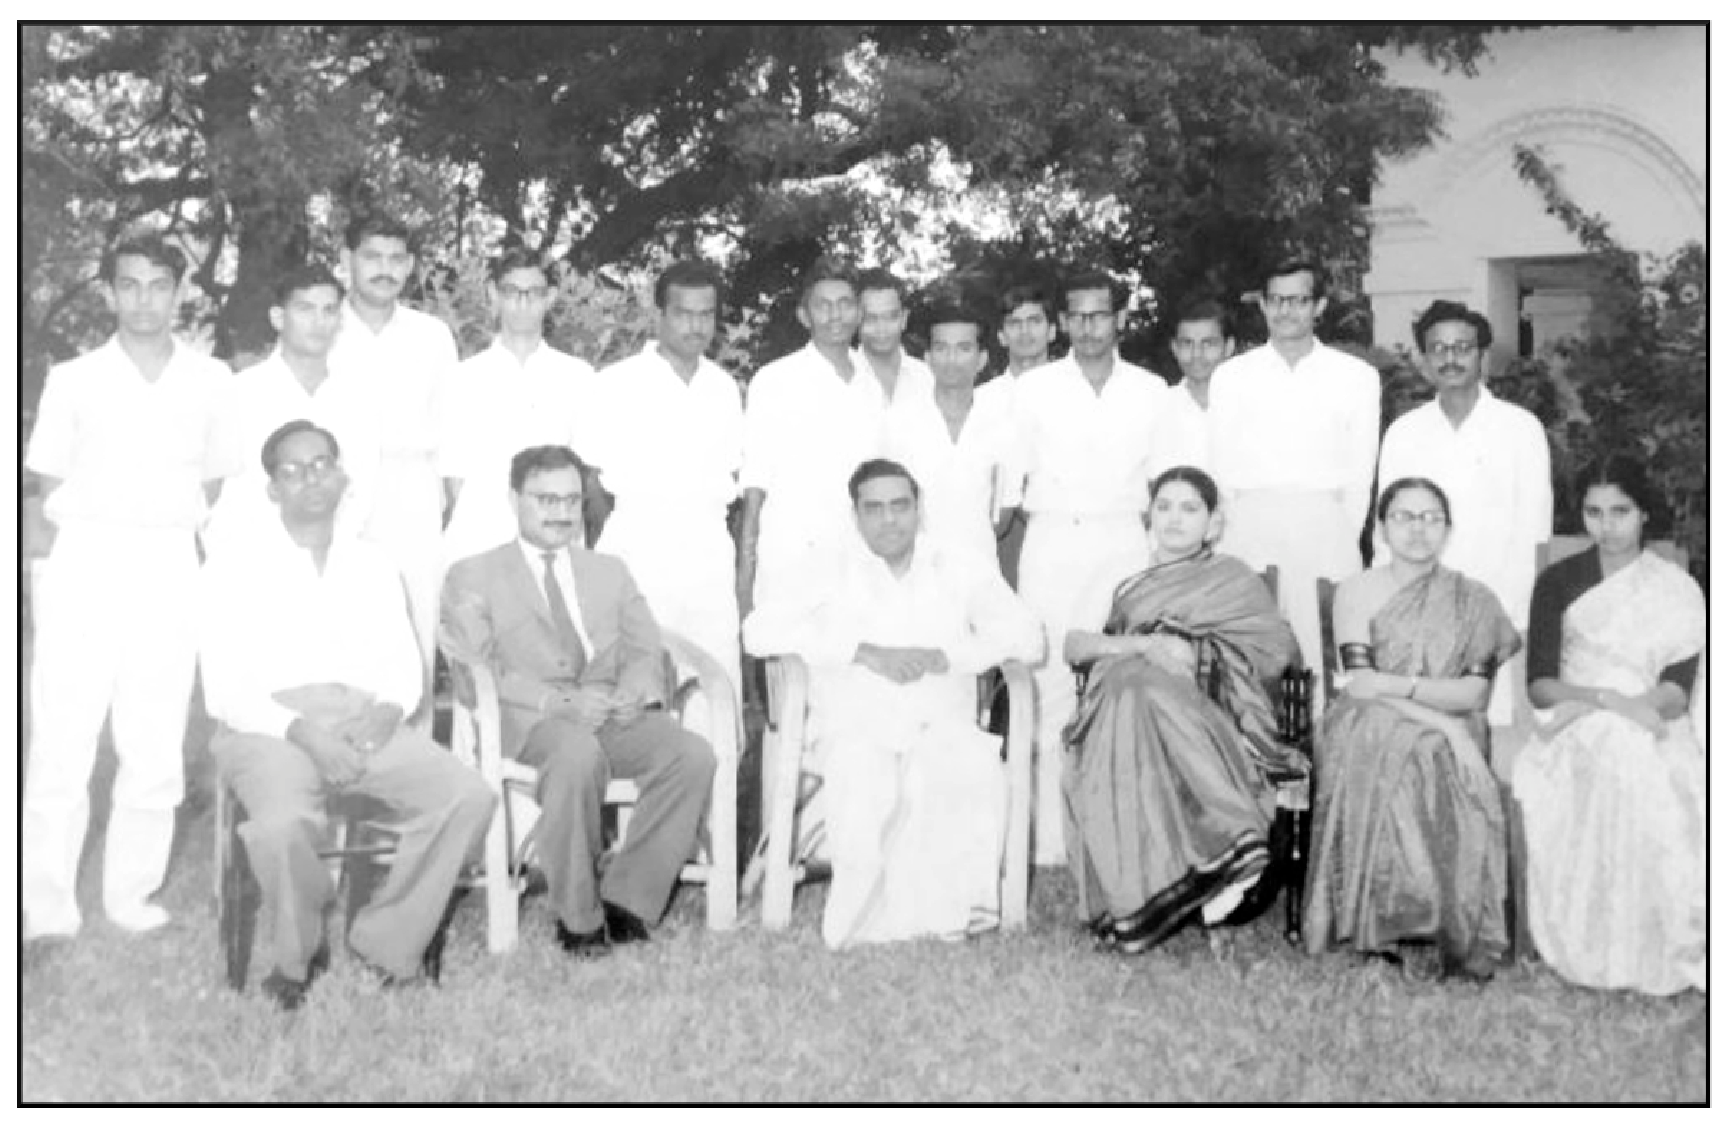
\includegraphics[scale=.32]{src/images/chap3/chap3-fig1.eps}\\
%~ \caption{Sitting: Dr.\ S. K. Srinivasan, Dr.\ Abdus Salam, Dr.\ A. Ramakrishnan, Mrs.\ Ramakrishnan, R. Thunga, T. K. Radha
%~ Standing: xxxxxxxxxxx V. Devanathan, G. Ramachandran}
%~ \end{figure}
%~ \medskip

%~ \begin{figure}[H]
%~ \centering
%~ 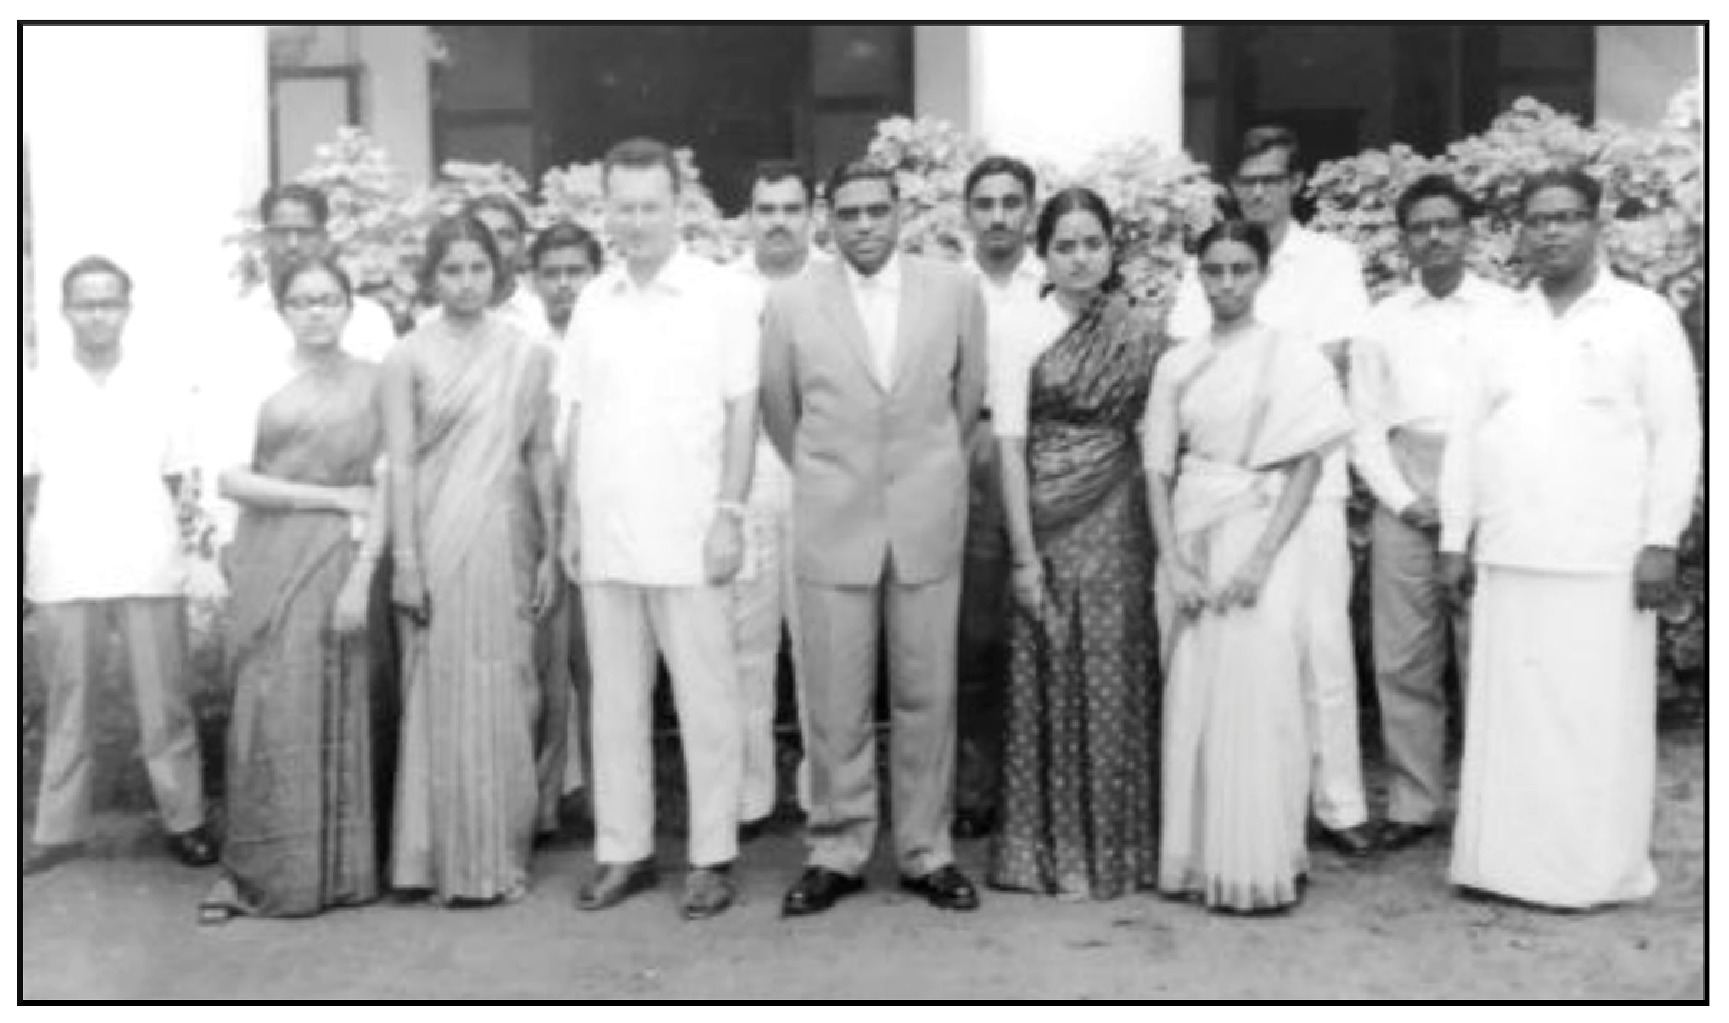
\includegraphics[scale=.32]{src/images/chap3/chap3-fig2.eps}\\
%~ \caption{Front Row: R. Thunga, T. K. Radha, Dr.\ Donald Glaser (N. L.), Dr.\ A. Ramakrishnan, S. Indhumathi, G. Bhamathi
%~ Second Row: A. P. Balachandran, K. Ananthanarayanan, K. Venkatesan, x, M.Deshpande, K. Raman, V. Devanathan, G. Ramachandran, Nambi Iyengar}
%~ \end{figure}

\begin{figure}[t]
\centering
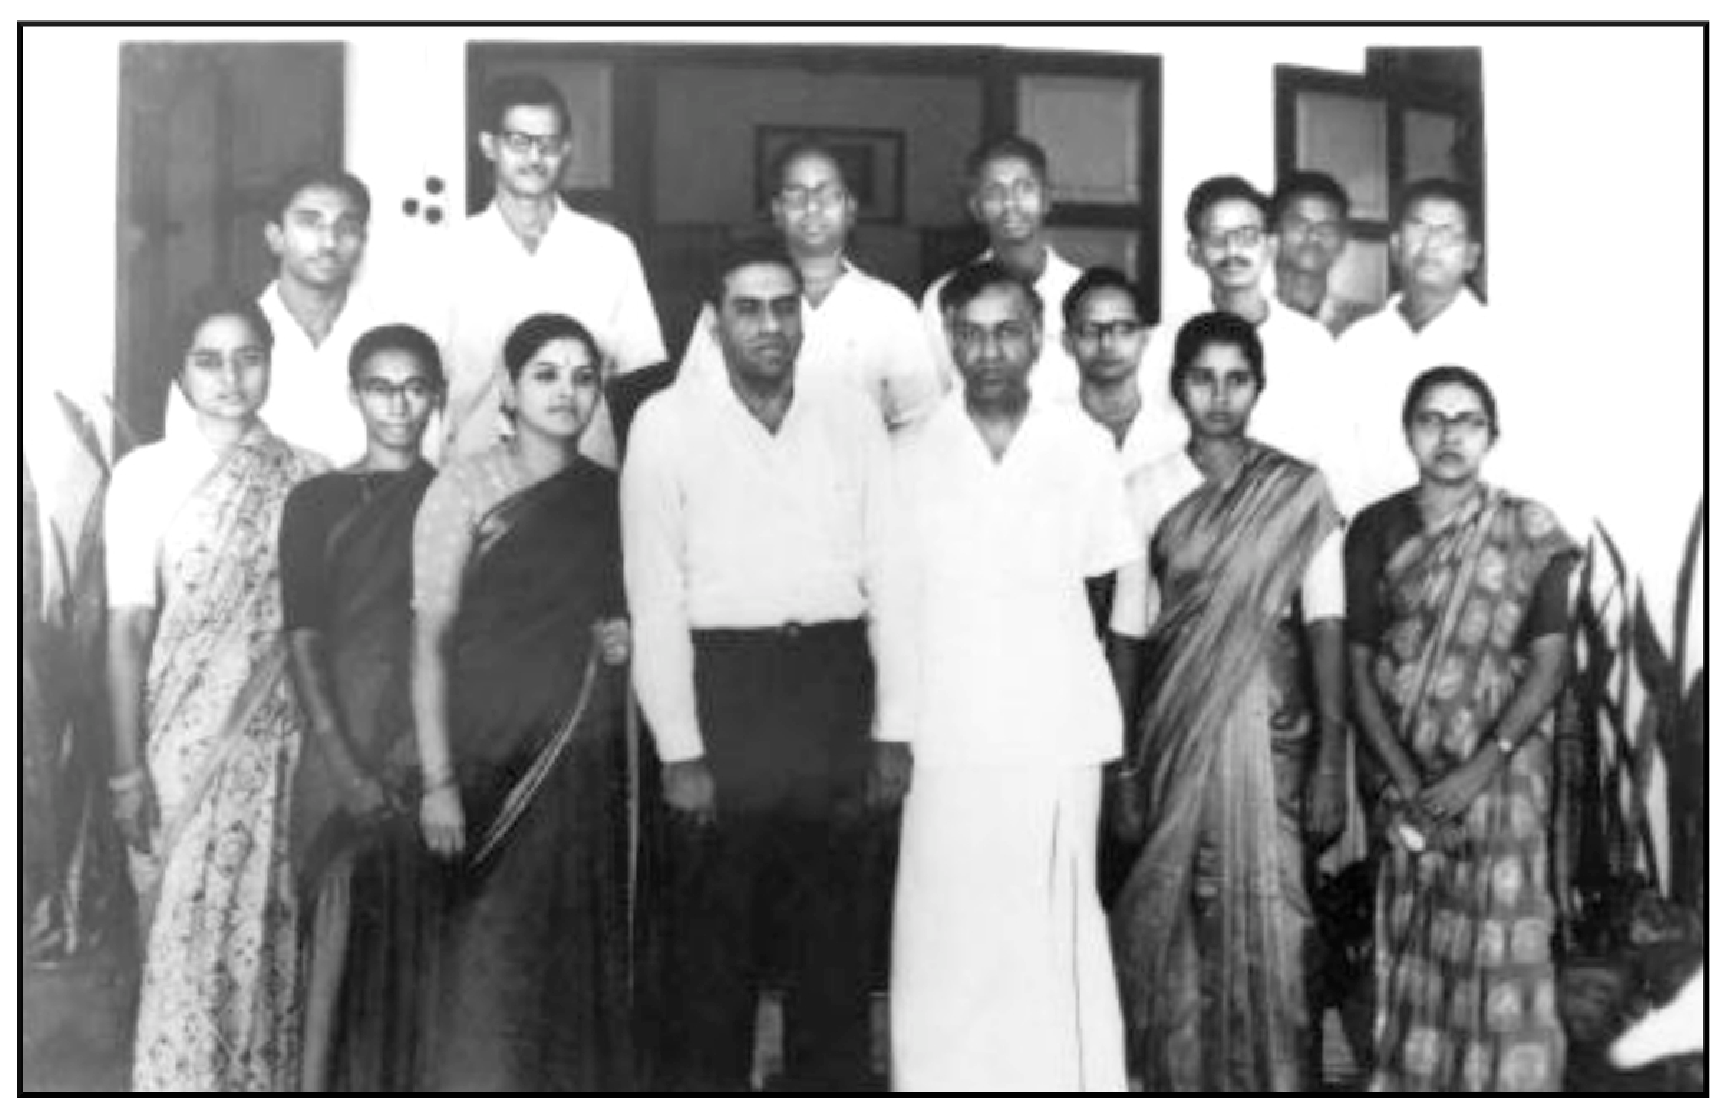
\includegraphics[scale=.35]{src/images/chap3/chap3-fig3.eps}\\
\caption{Front Row: S. Indhumathi, G. Bhamathi, Mrs.\ Ramakrishnan, Dr.\ A. Ramakrishnan, Dr.\ S. Chandrasekhar, T. K. Radha, R. Thunga;
Second Row: K. Raman, V. Devanathan, Dr.\ S. K. Srinivasan, K. Venkatesan, A. P. Balachandran, G. Ramachandran, x, Nambi Iyengar}
\end{figure}

At the Theoretical Physics Seminar, which was the forerunner of\break Institute of Mathematical Sciences, G. Ramachandran and I gave several lectures on different topics in Nuclear Physics. Prof.\ Manoj Banerjee from Calcutta University was invited by the Seminar and he gave a series of lectures on Angular Momentum. G. Ramachandran and I found those lectures very useful since the study of Nuclear physics involves a lot of angular momentum algebra. The investigation of static properties of nuclei such as magnetic dipole moment, electric quadrupole moment and the various energy levels of nuclei involve the calculation of matrix elements between nuclear states using the spherical tensor operators. The study of the dynamical properties of nuclei due to nuclear transition from one state to another as a result of interaction with external field is more involved since it requires the calculation of transition probability of nucleus from one state to another besides the evaluation of matrix elements. If the magnetic sub-states of the initial and final nuclei are not observed, we need to sum over the final magnetic sub-states and average over the initial magnetic sub-states. When we started our research, the study of elementary particle reactions with nuclei was an emerging field and it involved a knowledge of both elementary particle interactions and nuclear structure. Since angular momentum is a conserved quantity in any reaction, a sound knowledge of angular momentum algebra is a pre-requisite for such a study. This has motivated G. Ramachandran to publish the Matscience Report on Angular Momentum \cite{chap3-key10} and V. Devanathan, at a later date, to write Text Books, one on Angular Momentum \cite{chap3-key11} and another on Nuclear Physics \cite{chap3-key12}.

In the year 1957, Chew et al (hereafter referred to as CGLN) \cite{chap3-key13} has obtained a general amplitude for photoproduction of pions from nucleons using dispersion relations. Around the same time, Hughes and March \cite{chap3-key14} attempted to study experimentally the nuclear transitions to individual final nuclear states by observing the radioactivity of the final nuclear state. He studied the reaction ${}^{11} B(\gamma, \pi^-)^{11} C$. This was followed by other activity measurements by Dyal and Hummel \cite{chap3-key15} on ${}^{11} B$, by March and Walker \cite{chap3-key16} on ${}^{60} N i$, by Meyer et al \cite{chap3-key17} on ${}^{16} O$ and ${}^{27} Al$ and by Nydall and Forkman \cite{chap3-key18} on ${}^{11} B$, ${}^{27} Al$ and ${}^{51} V$.

Since the elementary amplitude for photoproduction of pion from nucleon was known and the experimental investigations on nuclei were already initiated, Ramachandran and I \cite{chap3-key4, chap3-key5} started to formulate a theory for photo-pion production from nuclei using impulse approximation and plane waves for the incident photon and the emitted pion.

The theoretical study of photoproduction of pions from nuclei depends on four essential factors:
\begin{enumerate}
\item The elementary photopion production amplitude for the nucleons
\item The construction of the nuclear transition amplitude from the free nucleon amplitude
\item The final state interaction of the outgoing pion with the residual nucleus
\item The nuclear structure
\end{enumerate}

One can check the validity of the elementary photopion production amplitude by comparing the calculated cross section with the experimentally observed cross section for the elementary process on free nucleons. This only checks the on-shell behaviour of the amplitude. In the nuclear process, the off-shell behaviour also counts. Besides, multiple scattering effects should also be considered. The plane wave approximation for the incident photon may be valid but definitely not for the pion. The calculated cross section with the plane wave approximation for the emitted pion was much larger than the experimental cross section and a phenomenological surface production model \cite{chap3-key19} was invoked to obtain the fit with experiment. Later on, The distortion effects on the emitted pion \cite{chap3-key20,chap3-key21} was properly taken into account by solving the Klein-Gordon equation with a suitable optical potential for the radial wave function. It was found that the nuclear structure also plays a vital part in the reaction.

Although our initial effort is to obtain an analytical expression for the photopion cross section from nuclei using simplifying assumptions, later we have found that the distortion effects on the pion and nuclear structure play a dominant role. A comprehensive review \cite{chap3-key22} on Photo-pions from nuclei is available. 

In this article, we do not follow the chronological order in the presentation but follow the logical sequence by discussing the coupling rule for spherical tensor operators, the evaluation of nuclear matrix elements and nuclear transition probability under the influence of spherical tensor operators \cite{chap3-key12}. The photo-pion production from nuclei is presented here for illustrative purpose only.

Both the static and dynamic properties of nuclei are studied by calculating nuclear matrix elements using spherical tensor operators. The coupling rules for spherical tensor operators are presented in Sec.\ \ref{chap3-sec2} as a prelude to the study of transition probability of nucleus from one state to another which is outlined in Sec.\ \ref{chap3-sec3}. In Sec.\ \ref{chap3-sec4}, we study the elementary photopion production reaction on nucleons. The study is extended to photopion production from nuclei in Sec.\ \ref{chap3-sec5.1} using impulse approximation for the reaction process and plane waves for the incident photon and the emitted pion. The plane wave approximation for the incident photon is justifiable but not for the outgoing pion. How to include the distortion effects on the emitted pion is discussed in Sec.\ \ref{chap3-sec5.2}.

\section{Coupling rules for Spherical Tensor Operators} \label{chap3-sec2}

The spherical harmaonics $Y^m_l(\theta, \phi)= Y_l^m (\hat{{\boldsymbol  r}})$ can be considered as spherical tensor operators and they obey the coupling rule
\begin{equation}
Y_{l_1}^{m_1} (\hat{{\boldsymbol  r}}) Y_{l_2}^{m_2} (\hat{{\boldsymbol  r}}) = \sum_L 
	\begin{bmatrix}
		l_1 & l_2 & L\\
		m_1 &m_2  & m_L
	\end{bmatrix}
(Y_{l_1} (\hat{{\boldsymbol  r}}) \times Y_{l_2} (\hat{{\boldsymbol  r}}))^{m_L}_{L}, \label{chap3-eq1}
\end{equation}
where
\begin{equation}
(Y_{l_1}  (\hat{{\boldsymbol  r}})  \times Y_{l_2} (\hat{{\boldsymbol  r}}) )^{m_L}_{L} = \frac{[l_1][l_2]}{\sqrt{4\pi}[L]}
\begin{bmatrix}
l_1 & l_2 & L\\
0 & 0 & 0
\end{bmatrix}
Y_{L}^{m_L} (\hat{{\boldsymbol  r}}). \label{chap3-eq2} 
\end{equation}
For brevity, the symbol $[l]$ is used to denote $[l]=\sqrt{2l+1}$. The wide square bracket represents the Clebsch-Gordan (C.G.) coefficient. For the notations and symbols, kindly refer to Devanathan \cite{chap3-key11,chap3-key12}. Eq.~\eqref{chap3-eq2} is applicable only to spherical harmonics but the definition \eqref{chap3-eq1} can be extended to any spherical tensor operators.

Let $A_{l_1}^{m_1}$ and $B_{l_2}^{m_2}$ be the components of any two spherical tensor operators of ranks $l_1$ and $l_2$. Then we can construct a tensor product $(A_{l_1} \times B_{l_2})^M_L$ using C.G. coefficients.
\begin{equation}
(A_{l_1} \times B_{l_2})^M_L = \sum_{m_1 ~m_2} 
\begin{bmatrix}
  l_1 & l_2 & L\\
  m_1 & m_2 & M
\end{bmatrix}
A_{l_1}^{m_1} B_{l_2}^{m_2}.  \label{chap3-eq3}
\end{equation}
In the special case In the special case of $L = 0$, we can write $l_1 = l_2 = l$ and $m_1 = -m_2 = m$ and the
tensor product can be expressed as a scalar product with a factor as shown in \eqref{chap3-eq4}.
\begin{align}
  (A_l \times B_l)^0_0 & = \sum_{m}
  \begin{bmatrix}  l & l & 0\\    m & -m & 0  \end{bmatrix}  A_l^m B_l^{-m}\notag\\
  & = \sum_m (-1)^{l-m} \frac{1}{[l]}
  \begin{bmatrix}    l & 0 & l\\    m & 0 & m  \end{bmatrix}  A_l^m B_l^{-m}\notag\\
  & = \frac{(-1)^l}{[l]} A_l \cdot B_l, \label{chap3-eq4}
\end{align}
using the notation $[l]=\sqrt{2l+1}$. One can write the inverse relation of \eqref{chap3-eq3}. Given any two spherical tensor operators $A_{l_1}^{m_1}$, $A_{l_2}^{m_2}$, they can be expressed as a linear sum of tensor products $(A_{l_1} \times B_{l_2})^M_L$, with $|l_1 -  l_2 | \leq L \leq l_1 + l_2$ 
\begin{equation}
A_{l_1}^{m_1} A_{l_2}^{m_2} = \sum_{L} 
\begin{bmatrix}
l_1 & l_2 &L\\
m_1 & m_2 & M
\end{bmatrix} (A_{l_1} \times B_{l_2})^M_L. \label{chap3-eq5}
\end{equation}

If there are three tensor operators $A_{l_1}$, $B_{l_2}$, $C_{l_3}$ , then it is possible to form a tensor product of them in more than one way: \eqref{chap3-eq1} by coupling $A_{l_1}$, $B_{l_2}$ and then coupling the resultant with $C_{l_3}$ or \eqref{chap3-eq2} by coupling $B_{l_2}$, $C_{l_3}$ first and then coupling $A_{l_1}$ with the resultant, as indicated below:
\begin{equation}
\left[ (A_{l_1} \times B_{l_2})_{l_{12}} \times C_{l_3}\right]^M_L;  \qquad \left[ A_{l_1} \times (B_{l_2} \times C_{l_3})_{l_{23}}\right]^M_L. \label{chap3-eq6}
\end{equation}
One can go from one coupling scheme to another by a unitary transformation,
\begin{align}
\left[ (A_{l_1} \times B_{l_2})_{l_{12}} \times C_{l_3}\right]^M_L  & = \sum_{l_{23}} U (l_1, l_2 L l_3, l_{12} l_{23})\notag \\ 
& \qquad \qquad \qquad \times \left[A_{l_1} \times (B_{l_2} \times C_{l_3})_{l_{23}} \right]^M_L. \label{chap3-eq7}\\ 
\left[ A_{l_1} \times (B_{l_2} \times C_{l_3})_{l_{23}}\right]^M_L & = \sum_{l_{12}} U (l_1, l_2 L l_3, l_{12} l_{23}) \notag \\
& \qquad \qquad \qquad \times \left[(A_{l_1} \times B_{l_2})_{l_{12}} \times C_{l_3}) \right]^M_L. \label{chap3-eq8} 
\end{align}
The unitary transformation coefficients $U (l_1 l_2 L l_3, l_{12} l_{23})$ defined in Eqs. \eqref{chap3-eq7} and \eqref{chap3-eq8} are exactly the recoupling coefficients that occur in the addition of three angular momenta \cite{chap3-key11,chap3-key12}. The recoupling coefficient $U (l_1 l_2 Ll_3 , l_{12} l_{23})$ can be expressed in terms of Racah coefficient $W (l_1 l_2 Ll_3 , l_{12} l_{23})$ 
\begin{equation}
U (l_1 l_2 Ll_3 , l_{12} l_{23}) = [l_{12}][l_{23}] W (l_{1} l_2 Ll_3 , l_{12} l_{23}). \label{chap3-eq9}
\end{equation}
If there are four spherical tensor operators $A_{l_1}, B_{l_2}, C_{l_3}, D_{l_4}$ of ranks $l_1, l_2,\break l_3, l_4$ respectively, then also one can construct tensor product of them in more than one way: \eqref{chap3-eq1} by coupling $A_{l_1}, B_{l_2}$ and $C_{l_3}, D_{l_4}$ separately to form tensors of rank $l_{12}$ and $l_{34}$ and then coupling these resultant tensors to form the product tensor of rank $L$ or \eqref{chap3-eq2} by coupling $A_{l_1}, C_{l_3}$ and $B_{l_2}, D_{l_4}$ initially to obtain the tensor products of rank $l_{13}$ and $l_{24}$ and then coupling these resultant tensors to obtain the product tensor of rank $L$. These two different ways of coupling correspond to two different representations and one can go from one representation to another representation by a unitary transformation, using the re-coupling coefficient. This is similar to the re-coupling coefficient that occur in the addition of four angular momenta \cite{chap3-key11,chap3-key12}.

\begin{align}
& [(A_{l_1} \times B_{l_2})_{l_{12}} \times (C_{l_3} \times D_{l_4})_{l_{34}}]^M_L \notag \\
& \qquad = \sum_{l_{13} l_{24}}
	\begin{bmatrix}l_1 & l_2 & l_{12}\\l_3 & l_4 & l_{34}\\l_{13} & l_{24} & L\end{bmatrix}
	\times [(A_{l_1} \times C_{l_3})_{l_{13}} \times (B_{l_2} \times D_{l_4})_{l_{24}}]^M_L. \label{chap3-eq10}\\
& [(A_{l_1} \times C_{l_3})_{l_{13}} \times (B_{l_2} \times D_{l_4})_{l_{24}}]^M_L  \notag \\
& \qquad = \sum_{l_{12} l_{34}}
	\begin{bmatrix}l_1 & l_2 & l_{12}\\l_3 & l_4 & l_{34}\\l_{13} & l_{24} & L\end{bmatrix} 
	\times [(A_{l_1} \times B_{l_2})_{l_{12}} \times (C_{l_3} \times D_{l_4})_{l_{34}}]^M_L. \label{chap3-eq11}
\end{align}
The recoupling coefficient (denoted by wide square brackets) that occurs in the coupling of four spherical tensors can be expressed in terms of Wigner's 9-j symbol (denoted by wide curly brackets).
\begin{equation}
	\begin{bmatrix}l_1 & l_2 & l_{12}\\l_3 & l_4 & l_{34}\\l_{13} & l_{24} & L\end{bmatrix} 
	= [l_{12}] [l_{34}] [l_{13}] [l_{24}] 
	\left\{\begin{matrix}l_1 & l_2 & l_{12}\\l_3 & l_4 & l_{34}\\l_{13} & l_{24} & L\end{matrix} \right\} \label{chap3-eq12}
\end{equation}

\subsection{Nuclear Matrix clements of spherical tensor operators}\label{chap3-sec2.1}

Let us now consider the evaluation of the following two-body matrix elements of spherical tensor operators:
\begin{align}
(1) ~ Q_1 & = \langle j_1' j_2' j' m' |A_k^\mu (1)| j_1 j_2 j m \rangle \label{chap3-eq13}\\
(2) ~ Q_2 & = \langle j_1' j_2' j' m' |B_k^\mu (2)| j_1 j_2 j m \rangle \label{chap3-eq14}\\
(3) ~ Q_3 & = \langle j_1' j_2' j' m' |(A_{k_1} (1) \times B_{k_2} (2))_k^\mu  | j_1 j_2 j m \rangle \label{chap3-eq15}
\end{align}

\medskip
\noindent \textbf{\large Evaluation by using recoupling coefficients}
\medskip

\noindent First let us evaluate the matrix element $Q_2$. Using the Wigner-Eckart theorem,
\begin{equation}
Q_2 = \begin{bmatrix}j & k & j'\\m & \mu & m'\end{bmatrix}
\langle j_1' j_2' j' || B_k (2) || j_1 j_2 j \rangle \delta_{j_1 j_1'}. \label{chap3-eq16}
\end{equation}
Since the operator acts on particle 2 only, the angular momentum of particle 1 is unaffected. In addition, the two-body reduced matrix element can be expressed in terms of one-body matrix element using the concept of recoupling coefficient $U$. The two-body matrix element corresponds to the coupling scheme of three angular momenta\footnote{The bold-face letters ${\boldsymbol  J}_1, {\boldsymbol  J}_2, {\boldsymbol  J}, \cdots$ are used to denote the angular momentum vectors whereas the corresponging lower case letters $j_1, j_2, j, \cdots$ denote the angular momentum quantum numbers.}
$$
{\boldsymbol  J}_1 + {\boldsymbol  J}_2 = {\boldsymbol  J}, \qquad {\boldsymbol  J}+ {\boldsymbol  K}= {\boldsymbol  J}',
$$
whereas the one-body marix element corresponds to the coupling scheme
$$
{\boldsymbol  J}_2 + {\boldsymbol  K} = {\boldsymbol  J}_2', \qquad {\boldsymbol  J}_1+ {\boldsymbol  J}_2'= {\boldsymbol  J}'.
$$
One can go from one coupling scheme to the other by using the unitary transformation coefficient $U(j_1 j_2 j' k, j j_2')$.
\begin{equation}
\langle j_1 j_2' j' || B_k (2) || j_1 j_2 j \rangle = U (j_1 j_2 j' k, j j_2') \langle j_2' || B_k (2) || j_2\rangle \label{chap3-eq17}
\end{equation}
Substituting \eqref{chap3-eq17} into Eq.\ \eqref{chap3-eq16}, we obtain
\begin{equation}
Q_2 = \begin{bmatrix}j & k & j'\\m & \mu & m'\end{bmatrix}
U (j_1 j_2 j' k, j j_2') \langle j_2' || B_k (2) || j_2\rangle \label{chap3-eq18}
\end{equation}

Having evaluated $Q_2$, we shall now evaluate $Q_1$. In $Q_1$, the transition operator $A_k^\mu$ \eqref{chap3-eq1} corresponds to particle 1. Switching particles 1 and 2 in the ket and bra vectors of two-particle system introduces a phase factor\footnote{The phase factor $(-1)^{j_1 +j_2-j}$ is either $+1$ or $-1$. This means $j_1 + j_2-j$ is either an even or odd integer.}  as shown below:
\begin{align}
| j_1 j_2 j m\rangle 
& = \sum_{m_1m_2} \begin{bmatrix}j_1 & j_2 & j\\m_1 & m_2 & m\end{bmatrix} |j_1 m_1 \rangle| j_2 m_2\rangle \notag \\
& = (-1)^{j_1+j_2-j} \sum_{m_1 m_2} 
	\begin{bmatrix}j_2 & j_1 & j\\m_2 & m_1 & m \end{bmatrix} |j_1 m_1 \rangle | j_2 m_2 \rangle \notag \\
& = (-1)^{j_1 + j_2-j} | j_2 j_1 j m \rangle .\label{chap3-eq19}
\end{align}
Similarly,
\begin{equation}
|j_1' j_2 j' m' \rangle = (-1)^{j_1' + j_2 - j'} | j_2 j_1' j' m' \rangle . \label{chap3-eq20}
\end{equation}
Hence\footnote{The product of two phase factors $(-1)^{n_1} (-1)^{n_2}$ can be written either as $(-1)^{n_1 + n_2}$ or as $(-1)^{n_1-n_2}$, since $n_1$ and $n_2$ are integers (either odd or even).}
\begin{eqnarray}
	Q_1 &=& (-1)^{j_1+j_2-j}(-1)^{j_1'+j_2-j'}
\left[ \begin{array}{ccc}
		j & k & j'\\
		m & \mu & m'  \end{array} \right] 
\langle j_2\, j_1'\, j'\, || A_k(1) || j_2\, j_1\,j\,\rangle\nonumber \\
	&=& (-1)^{j_1-j_1'-j+j'}
	\left[ \begin{array}{ccc}
		j & k & j'\\
		m & \mu & m'  \end{array} \right] 
	\langle j_2\, j_1'\, j'\, || A_k(1) || j_2\, j_1\,j\,\rangle \nonumber \\
	&=& (-1)^{j_1-j_1'-j+j'}
	\left[ \begin{array}{ccc}
		j & k & j'\\
		m & \mu & m'  \end{array} \right] U(j_2\,j_1\,j'\, k\,,\,j\,j_1')\,
	\langle j_1'\, || A_k(1) ||  j_1\,\rangle.
\nonumber \\
	\label{chap3-eq21}
\end{eqnarray}
The last step is obtained using Eq.\ \eqref{chap3-eq17}. Only the subscripts 1 and 2 are interchanged. 

We shall now evaluate $Q_3$. Applying the Wigner-Eckart theorem,
\begin{equation}
  Q_3 =
  \begin{bmatrix}    j & k & j'\\    m & \mu & m'  \end{bmatrix}
  \langle j_1' j_2' j' || (A_{k_1}(1) \times B_{k_2}(2))_k || j_1 j_2 j \rangle. \label{chap3-eq22}
\end{equation}
The double-bar matrix element is independent of the coordinate system. It is a two-particle matrix element and it can be expressed as a product of two one-particle matrix elements by going from one coupling scheme (a) to another coupling scheme (b) by unitary transformation.
\begin{alignat*}{3}
  (a) \quad&  {\boldsymbol  J}_1 + {\boldsymbol  J}_2 = {\boldsymbol  J}, \qquad &{\boldsymbol  K}_1+ {\boldsymbol  K}_2= {\boldsymbol  K}, \qquad &{\boldsymbol  J} + {\boldsymbol  K}= {\boldsymbol  J}'.\\
  (b) \quad &{\boldsymbol  J}_1 + {\boldsymbol  K}_1 = {\boldsymbol  J}_1', \qquad &{\boldsymbol  J}_2+{\boldsymbol  K}_2= {\boldsymbol  J}_2', \qquad & {\boldsymbol  J}_1'+{\boldsymbol  J}_2'={\boldsymbol  J}'.
\end{alignat*}
\begin{align}
  \langle j_1' j_2' j' || & (a_{k_1}(1) \times B_{k_2}(2))_k ||  j_1 j_2 j \rangle \notag \\
  & =  \begin{bmatrix} j_1 & j_2 & j\\ k_1 & k_2 & k \\ j_1' & j_2' & j'  \end{bmatrix}
  \langle j_1' || A_{k_1}(1)|| j_1 \rangle \times \langle j_2' || B_{k_2} (2)|| j_2 \rangle . \label{chap3-eq23}
\end{align}

\section{Nuclear Transition Probability}\label{chap3-sec3}

Let us consider the transition of a nucleus from an initial state $|j_l m_i \rangle$ to a final state $| j_f m_f \rangle$ due to the interaction with an external field. If $H_I$ is the interaction Hamiltonian, then the transition probalility is given by
\setcounter{equation}{23}
\begin{equation}
  T_{fi} = \frac{1}{2j_i +1} \sum_{m_i m_f} | \langle j_f m_f |H_I| j_i m_i \rangle |^2, \label{chap3-eq24}
\end{equation}
where a sum over the final spin states and an average over the initial spin states have been taken. The interaction Hamiltonian $H_I$ which is a scalar can be expressed as a scalar product of two tensors, one corresponding to the external field and the other corresponding to the nuclear field.
\begin{equation}
  H_I = \sum_{\lambda m_\lambda} (A_\lambda^{m_\lambda})^\ast U_\lambda^{m_\lambda}, \label{chap3-eq25}
\end{equation}
where $U_\lambda^{m_\lambda}$ is the spherical tensor operator in nuclear coordinates inducing nuclear transition and $A_\lambda^{m_\lambda}$ is the spherical tensor component of the external field. Substituting \eqref{chap3-eq25} into Eq.\ \eqref{chap3-eq24}, we obtain
\begin{eqnarray}
T_{fi} &=&  \frac{1}{2j_i +1}\sum_{m_i m_f}\left| \sum_{\lambda m_{\lambda}}
\left(A_\lambda^{m_\lambda}\right)^*
\langle j_f m_f| U_\lambda^{m_\lambda}|j_i m_i \rangle \right|^2
\nonumber \\
&=& \frac{1}{2j_i +1}\sum_{m_i m_f} \sum_{\lambda \lambda' m_\lambda
	m_\lambda'}\left( A_\lambda^{m_\lambda}\right)^* A_{\lambda'}^{m_\lambda'}\nonumber\\
& &\times \langle j_f m_f|U_\lambda^{m_\lambda}| j_i m_i \rangle
\langle j_f m_f|U_{\lambda'}^{m_\lambda'}| j_i m_i \rangle^*.
\label{chap3-eq26}
\end{eqnarray}
The dependence of the nuclear matrix element on magnetic quantum numbers can be factored out as a C.G. coefficient, using the Wigner-Eckart theorem.
\begin{equation}
  \langle j_f m_f | U_\lambda^{m_\lambda}| j_i m_i\rangle =
  \begin{bmatrix} j_i & \lambda & j_f\\ m_i & m_\lambda & m_f \end{bmatrix} \langle j_f || U_\lambda|| j_i \rangle . \label{chap3-eq27}
\end{equation}
Applying the Wigner-Eckart theorem, we get
\begin{align}
  T_{fi}  = & \frac{1}{2j_i+1} \sum_{m_i m_f} \sum_{\lambda \lambda' m_\lambda m_\lambda'} (A_\lambda^{m_\lambda})^\ast A_{\lambda'}^{m_\lambda'}
  \notag \\
 &  \begin{bmatrix} j_i & \lambda & j_f \\ m_i & m_\lambda & m_f\end{bmatrix}
    \begin{bmatrix} j_i & \lambda' & j_f \\ m_i & m_\lambda' & m_f\end{bmatrix}
      \times \langle j_f || U_\lambda || j_i \rangle \langle j_f || U_{\lambda'} || j_i \rangle^\ast. \label{chap3-eq28}
\end{align}
Summing over $m_i$ and using the orthonormal properties of the C.G. coefficients, we get
\begin{align}
  \sum_{m_i} &
  \begin{bmatrix} j_i & \lambda & j_f\\ m_i & m_\lambda & m_f  \end{bmatrix}
  \begin{bmatrix} j_i & \lambda' & j_f \\ m_i & m_\lambda' & m_f\end{bmatrix} \notag \\
    & = \sum_{m_i} \frac{[j_f]^2}{[\lambda][\lambda']}
      \begin{bmatrix} j_i &  j_f  & \lambda \\ m_i &  -m_f & -m_\lambda\end{bmatrix}
      \begin{bmatrix} j_i &  j_f  & \lambda' \\ m_i &  -m_f & -m_\lambda'\end{bmatrix} \notag \\
    & = \frac{[j_f]^2}{[\lambda][\lambda']} \delta_{\lambda \lambda'} \delta_{m_\lambda m_\lambda'}, \label{chap3-eq29}    
\end{align}
using the notation
$$
[\lambda] = \sqrt{2 \lambda +1}.
$$
Substituting \eqref{chap3-eq29} into Eq.\ \eqref{chap3-eq28} and summing over $\lambda'$ and $m_\lambda'$, we obtain (summation over $m_f$ is redundant)
\begin{align}
  T_{f_i} & = \frac{1}{2j_i +1} \sum_{\lambda m_\lambda} \frac{[j_f]^2}{[\lambda]^2} (A_\lambda^{m_\lambda})^\ast A_\lambda^{m_\lambda} \langle j_f || U_\lambda || j_i \rangle \langle j_f || U_\lambda || j_i \rangle^\ast \notag \\
  & = \frac{2j_f+1}{2j_i+1} \sum_{\lambda} \frac{1}{[\lambda]^2} (A_\lambda^\ast \cdot A_\lambda)| \langle j_f || U_\lambda || j_i \rangle |^2. \label{chap3-eq30}
\end{align}
Eq.\ \eqref{chap3-eq30} gives the nuclear transition probability in any reaction. Let us apply this formalism to the study of photopion reaction for illustrative purpose.

\section{Elementary photopion production cross section}\label{chap3-sec4}

Let us consider the reaction
$$
\gamma + p \to \pi^+ + n.
$$
Since the nucleon spin is $\frac{1}{2}$, the production amplitude will partly depend on spin and partly be independent of spin. Denoting the spin dependent part by ${\boldsymbol  K}$ and spin-independent part by $L$, we can write the transition operator as
\setcounter{equation}{30}
\begin{equation}
t= ({\boldsymbol  \sigma \cdot K} + L) e^{i(\boldsymbol  \nu- \mu)\cdot {\boldsymbol  r}/\hbar}= ({\boldsymbol  \sigma \cdot K} + L) e^{i {\boldsymbol  q \cdot r}/\hbar}, \label{chap3-eq31}
\end{equation}
where $\boldsymbol{\sigma}$ is the Pauli spin operator. The incident photon and the outgoing pion are represented by plane waves $e^{i\nu  \cdot r/\hbar}$ and $e^{-i \mu \cdot r /\hbar}$ and ${\boldsymbol  q}$ denotes the momentum transfer to the nucleon. The matrix element for transition of the nucleon from the initial state $|\frac{1}{2}, m_i \rangle$ to the final state $|\frac{1}{2}, m_f \rangle$ is given by
\begin{equation}
  M_{fi} = \langle \tfrac{1}{2}, m_f | {\boldsymbol  \sigma \cdot K} + L | \tfrac{1}{2}, m_i \rangle e^{i {\boldsymbol  q \cdot r}/\hbar}. \label{chap3-eq32}
\end{equation}
This is the transition amplitude and the transition probability $T_{fi}$ is given by the modulus square $|M_{fi}|^2$, obtained after summing over the final spin state and averaging over the initial spin state.
\begin{align}
  T_{fi} & = \frac{1}{2} \sum_{m_i, m_f} | \langle \tfrac{1}{2}, m_f | {\boldsymbol  \sigma \cdot K} + L | \tfrac{1}{2}, m_i\rangle|^2 \notag \\
  & = \frac{1}{2} \sum_{m)i, m_f} (\langle \tfrac{1}{2}, m_f | {\boldsymbol  \sigma. \cdot K + L}| \tfrac{1}{2}, m_i \rangle) \langle \tfrac{1}{2}, m_f | {\boldsymbol  \sigma, K + L}| \tfrac{1}{2}, m_i \rangle^\dagger \notag\\
  & = \frac{1}{2} \sum_{m_i, m_f} \langle \tfrac{1}{2}, m_f + {\boldsymbol  \sigma \cdot K} + L | \tfrac{1}{2}, m_i \rangle \langle \tfrac{1}{2} , m_i | {\boldsymbol  \sigma \cdot K^\ast}+ L^\ast| \tfrac{1}{2}, m_f \rangle \notag\\
  & = \frac{1}{2} \sum_{m_f} \langle \tfrac{1}{2}, m_f | ({\boldsymbol  \sigma \cdot K} + L) ({\boldsymbol  \sigma \cdot K^\ast} + L^\ast) | \tfrac{1}{2}, m_f \rangle,\notag\\
  & \qquad \qquad \qquad \qquad \qquad ~\text{since}~ \sum_{m_i} |\tfrac{1}{2}, m_i \rangle \langle \tfrac{1}{2}, m_i| =1 \notag\\
  & = \frac{1}{2} ~\text{Tr}~  \{ ({\boldsymbol  \sigma \cdot K}+L)({\boldsymbol  \sigma \cdot K^\ast}
  + L^\ast)\}\notag \\
  & = {\boldsymbol  K \cdot K^\ast} + LL^\ast \label{chap3-eq33}
\end{align}
In deducing Eq.\ \eqref{chap3-eq33}, we have used the Hermitian property of the $2 \times 2$ Pauli matrices $\sigma_x, \sigma_y, \sigma_z$ with trace zero.
$$
\sigma^\dagger = \sigma; \quad \text{Tr}~ \sigma_x = \text{Tr}~ \sigma_y = \text{Tr}~ \sigma_z =0.
$$
In addition,
\begin{alignat*}{3}
  &({\boldsymbol  \sigma \cdot K}) ({\boldsymbol  \sigma \cdot K}^\ast) = {\boldsymbol  K \cdot K}^\ast && +  i{\boldsymbol  \sigma \cdot (K \times K^\ast)}\\
  & \text{Tr}~  ({\boldsymbol  \sigma \cdot K})L^\ast =0; && \text{Tr}~ \sigma \cdot ({\boldsymbol  K \times K}^\ast)=0\\
  & \text{Tr}~ {\boldsymbol  K \cdot K}^\ast = 2 {\boldsymbol  K \cdot K}^\ast; & &\text{Tr}~LL^\ast = 2LL^\ast.
\end{alignat*}

The transition probability $T_{fi}$ given by Eq.\ \eqref{chap3-eq33} is energy-dependent and one can obtain the transition probability per unit time $Q_{fi}$ for photo-pion prosuvtion, using Fermi's Golden rule \cite{chap3-key23}.
\begin{equation}
  Q_{fi}= \frac{2 \pi}{\hbar} T_{fi}\, \rho_f, \label{chap3-eq34}
\end{equation}
where $\rho_f$ denotes the density of final states of pions.

\subsection{Density of final states}\label{chap3-sec4.1}

The state of a particle is defined by defining its position and momentum simultaneously at a given time. In classical physics, there is no restriction on their precise determination and so the state of a particle can be represented by a point on the six-dimensional phase-space which is a product of ordinary space and momentum space. But, in quantum physics, the state of a particle can only be represented by a cell of volume $h^3$ in phase-space \cite{chap3-key24}, since the position and momentum are canonically conjugate variables. According to Heisenberg's uncertainty principle, the uncertainty in measuring each pair of components is $\Delta x \Delta p_x \sim h$, $\Delta y \Delta p_y \sim h$, $\Delta z \Delta p_z \sim h$, where $h$ denotes the Planck constant. So, the number of quantal states that are possible for a particle in volume $V$ with momentum lying between $p$ and $p + dp$ is obtained from phase-space consideration \cite{chap3-key24} is
$$
N = \frac{Vp^2 dpd\Omega}{h^3}.
$$
This can be expressed in terms of energy. If $m$ is the rest mass of the particle, then its relativistic energy $E$ is given by the relation $E^2= p^2 c^2+ m^2 c^4$, which, on defferentiation, yields the relation $EdE=c^2pdp$. In terms of energy
$$
N= \frac{Vp{EdE}}{c^2 h^3},
$$
where $h$ denotes the Planck constant and $c$, velocity of light. Thus, we obtain the density of states
$$
\rho = \frac{N}{V} = \frac{p{EdE}}{c^2 h^3} = \frac{p{EdE}}{c^2 (2\pi \hbar)^3},
$$
where $\hbar = \tfrac{h}{2\pi}$.

\subsection{Differential cross section}\label{chap3-sec4.2}

The cross section depends on the incident flux. In this case, the number of photons incident on unit area of the target is $c$, using the usual normalization of one particle per unit volume.
\begin{align}
  \text{Cross section}~ & = \frac{Q_{fi}}{\text{Incident flux}} = \frac{Q_{fi}}{c}\notag \\
  & = \frac{2 \pi}{\hbar c} T_{fi} \rho_ f \notag \\
  & = \frac{2\pi}{\hbar c} T_{fi} \frac{\mu \mu_0 d \mu_0 d \Omega}{c^2 (2 \pi \hbar)^3},\label{chap3-eq35}
\end{align}
where $\mu$ denotes the outgoing pion momentum and $\mu_0$, its relativistic energy (including the rest mass energy; $\mu_0^2 = \mu^2 c^2 + m_\pi^2 c^4$). The integral over $d\mu_0$ yields the muon energy ($\mu_0$) in the final state to be equal to the incident photon energy ($\nu_0$). It is convenient to use natural units $\hbar =1$, $c=1$, $m_\pi =1$. In natural units, the differential cross section becomes
\begin{align}
  \frac{d \sigma}{d \Omega} & = (2 \pi)^{-2} \mu \mu_0 T_{fi}\notag \\
  & = (2 \pi)^{-2} \mu \mu_0 ({\boldsymbol  K^\ast \cdot K} + L^\ast L) \label{chap3-eq36}
\end{align}
Eq.\ \eqref{chap3-eq36} represents the differential cross section for the elementary process of photoproduction of pions from nucleons.

\section{Photoproduction of pions from nuclei}\label{chap3-sec5}

\subsection{Plane wave approximation for emitted pion}\label{chap3-sec5.1}

Let us now consider the transition of a bound nucleon from an initial state $|R_i (r)$, $l_i \frac{1}{2} j_i m_i \rangle$ to a final state $|R_f (r)$, $l_f \frac{1}{2} j_f m_f \rangle$ due to the interaction with an external field. Using the plane wave approximation for the incident photon and the emitted pion, the transition operator can be written as (in natural units with $\hbar =1$, $c=1$)
\setcounter{equation}{36}
\begin{equation}
  t_{op}= e^{-i {\boldsymbol  \mu \cdot r}} ({\boldsymbol  \sigma \cdot K} + L)e^{i {\boldsymbol  \nu \cdot r}}= ({\boldsymbol  \sigma \cdot K}+ L) e^{i ({\boldsymbol  \nu - \mu})\cdot {\boldsymbol  r}} \label{chap3-eq37}
\end{equation}
If we treat the spin-dependent and spin-independent parts of the amplitude alike by defining an unit operator $\sigma_0$ in spin space and redefining ${\boldsymbol  K}$ and $L$ by ${\boldsymbol  K_1}$ and $K_0$ , we can write the transition operator in a form, suitable for evaluation of the matrix element.
\begin{align}
  t_{op} = \sum_{0, 1} \sigma_n \cdot {\boldsymbol  K}_n e^{i{\boldsymbol  q \cdot r}}, \label{chap3-eq38}
\end{align}
where $q= \nu- \mu$ is the momentum transfer. Expanding $e^{i {\boldsymbol  q \cdot r}}$ into partial waves,
\begin{equation}
  e^{i {\boldsymbol  q \cdot r}} = 4 \pi \sum_{lm} (i)^l j_l (qr) (-1)^{m}Y_l^m (\hat{{\boldsymbol  r}}) Y_l^{-m} (\hat{{\boldsymbol  q}}), \label{chap3-eq39}
\end{equation}
Where $j_l (qr)$ represents the spherical Bessel functions. the transition operator can now be written as
\begin{equation}
 t_{op}= 4 \pi \sum_{lm} (i)^l j_l (qr) (-1)^m Y_l^m (\hat{{\boldsymbol  r}}) Y_l^{-m} (\hat{{\boldsymbol  q}}) \sum_{n\mu} (-1)^\mu {\boldsymbol \sigma}_n^\mu {\boldsymbol K}_n^{-\mu}. \label{chap3-eq40}
\end{equation}
Separating the nuclear operators from the rest and forming tensor products in pairs,
\begin{align}
  Y_l^m ({\boldsymbol \hat{r}}) {\boldsymbol \sigma}_n^\mu & = \sum_{\lambda}
  \begin{bmatrix} L & n & \lambda\\ m & \mu & m_\lambda \end{bmatrix} (Y_l ({\boldsymbol \hat{r}}) \times {\boldsymbol \sigma_n})_\lambda^{m_\lambda}. \label{chap3-eq41}\\
  Y_l^{-m} ({\boldsymbol \hat{q}}) {\boldsymbol K}_n^{-\mu} & = \sum_{\lambda'}
  \begin{bmatrix}    l & n & \lambda' \\ -m & -\mu & -m_\lambda  \end{bmatrix}
  (Y_l ({\boldsymbol \hat{q}}) \times {\boldsymbol K}_n)_{\lambda'}^{-m_\lambda} \notag \\
  & = \sum_{\lambda '} (-1)^{l + n - \lambda'}
  \begin{bmatrix}    l & n & \lambda'\\ m & \mu & m_\lambda  \end{bmatrix}
  (Y_l ({\boldsymbol \hat{q}}) \times {\boldsymbol K}_n)_{\lambda'}^{-m_\lambda}. \label{chap3-eq42}
\end{align}
Substituting \eqref{chap3-eq41} and \eqref{chap3-eq42} into Eq.\ \eqref{chap3-eq40} and summing over the projection quantum number $m$, the orthonormality of C.G. coefficients yields $\delta_{\lambda \lambda'}$. Replacing the summation over $\mu$ by $m_{\lambda}$, the transition operator \eqref{chap3-eq40} becomes
\begin{align}
  t_{op} & = 4 \pi \sum_{ln \lambda m_\lambda} (i)^l j_l (qr) (-1)^{l + n - \lambda} (-1)^{m_\lambda} (Y_l({\boldsymbol \hat{r}}) \times \sigma_n)_\lambda^{m_\lambda} (Y_l ({\boldsymbol \hat{q}}) \times {\boldsymbol K}_n)_\lambda^{-m_\lambda} \notag \\
  & = 4 \pi \sum_{ln \lambda m_\lambda} (i)^l j_l (qr) (-1)^{l+n-\lambda} (Y_l ({\boldsymbol \hat{r}}) \times \sigma_{n})_\lambda \cdot (Y_l ({\boldsymbol \hat{q}}) \times {\boldsymbol K}_n)_\lambda. \label{chap3-eq43}
\end{align}

The matrix element $M_{fi}$ of the transition operator $t_{\text{op}}$ taken between the initial and final nuclear states\footnote{The bound state of the nucleon is represented by $|R(r), l \tfrac{1}{2} jm \rangle$, where $R(r)$ denotes the radial part and $|l\tfrac{1}{2} jm \rangle$ denotes the angular part.} is the transition amplitude.
\begin{align}
  M_{fi} & = \langle R_f (r), l_f \tfrac{1}{2} j_f m_f| t_{\text{op}}| R_i (r) , l_i \tfrac{1}{2} j_i m_i \rangle \notag \\
  & = 4 \pi \sum_{ln\lambda m_\lambda} (i)^l (-1)^{l + n -\lambda} (-1)^{m_\lambda} (Y_l ({{\hat{\boldsymbol q}}}) \times {\boldsymbol K}_n)_{\lambda}^{-m_\lambda} \notag \\
  & \qquad \times \langle R_f (r), l_f \tfrac{1}{2} j_f m_f | j_l (qr) (Y_l ({\boldsymbol \hat{r}}) \times \sigma_n)_\lambda^{m_\lambda} |R_i (r), l_i \tfrac{1}{2} j_i m_i \rangle \notag \\
  & = 4\pi \sum_{ln \lambda m_\lambda} (i)^l (-1)^{l + n -\lambda} (-1)^{m \lambda} (Y_l({\boldsymbol \hat{q}})\times {\boldsymbol K}_n)^{-m_\lambda}_\lambda \langle j_l (qr)\rangle_{fi}\notag \\
  &\quad\times \begin{bmatrix} j_i & \lambda & j_f \\ m_i & m_\lambda & m_f \end{bmatrix}
  \langle l_f \tfrac{1}{2} j_f || (Y_l ({\boldsymbol \hat{r}}) \times \sigma_n)_\lambda|| l_i \tfrac{1}{2} j_i \rangle, \label{chap3-eq44}
\end{align}
where
$$
\langle j_l (qr)\rangle_{fi} = \int R_f (r)^\ast j_l(qr) R_i (r) r^2 dr
$$
is the radial integral. The C.G. coefficient in Eq.\ \eqref{chap3-eq44} is obtained by the application of Wigner-Eckart theorem.

The matrix element is a linear sum of several terms and so its square will include cross terms also. Hence
\begin{align}
  |M_{fi}|^2 & = 16\pi^2 \sum_{ln\lambda m_\lambda} \sum_{l' n' \lambda' m_\lambda '} (i)^{l-l'} (-1)^{l + n - \lambda} (-1)^{l' + n' \lambda'} (-1)^{m\lambda} (-1)^{m_\lambda'} \notag \\
  &  \quad \times (Y_l ({\boldsymbol \hat{q}}) \times {\boldsymbol K}_n)_\lambda^{-m\lambda}  \left\{ (Y_{l'} ({\boldsymbol \hat{q}}) \times {\boldsymbol K}_{n'})_{\lambda'}^{-m_\lambda'}\right\}^\ast \langle j_l (qr)\rangle_{fi} \langle j_{l'}(qr)\rangle^\ast_{f_i} \notag \\
  & \quad \times \begin{bmatrix} j_i & \lambda & j_f\\ m_i & m_\lambda & j_f \end{bmatrix}
  \langle l_f \tfrac{1}{2} j_f || (Y_l ({\boldsymbol \hat{r}}) \times \sigma_n)_\lambda || l_i \tfrac{1}{2} j_i \rangle \notag \\
  & \quad \times \begin{bmatrix} j_i & \lambda' & j_f\\ m_i & m_\lambda' & m_f \end{bmatrix}
  \langle l_f \tfrac{1}{2} j_f || (Y_{l'} ({\boldsymbol \hat{r}}) \times \sigma_{n'})_{\lambda'} || l_i \tfrac{1}{2} j_i \rangle^\ast. \label{chap3-eq45}
\end{align}
Summing over the final spin states and averaging over the initial spin states, we obtain the transition probability.
\begin{equation}
  T_{fi} = \frac{1}{2j_i +1} \sum_{m_i m_f} |M_{fi}|^2. \label{chap3-eq46}
\end{equation}
Summing over $m_i$ and using the orthonormality of C.G. coefficients as shown in \eqref{chap3-eq29}, we obtain the relations $\lambda = \lambda'$ and $m_\lambda= m_\lambda'$. Of the summations $m_f$ and $m_\lambda$, one is redundant since $m_f= m_i+ m_\lambda$. Substituting the results \eqref{chap3-eq29} and \eqref{chap3-eq45} into Eq.\ \eqref{chap3-eq46}, we obtain the transition probalility $T_{fi}$.
\begin{align}
  T_{fi} & = 16\pi^2 \frac{2j_f +1}{2j_i+1} \sum_{lnl'n'} \sum_{\lambda m_\lambda} \frac{1}{[\lambda]^2} (i)^{l-l'} (-1)^{l+ n - \lambda} (-1)^{l' + n'-\lambda}\notag \\
  &  \times (Y_l ({\boldsymbol \hat{q}}) \times {\boldsymbol K}_n)^{-m\lambda}_\lambda \left\{ (Y_{l'}({\boldsymbol \hat{q}}) \times {\boldsymbol K}_{n'})_\lambda^{-m_\lambda}\right\}^\ast \langle j_l (qr)\rangle_{f_i} \langle j_{l'}(qr)\rangle_{f_i}^\ast \notag \\
  &  \times \langle l_f \tfrac{1}{2} j_f || (Y_l (({\boldsymbol \hat{r}}) \times \sigma_n)_\lambda || l_i \tfrac{1}{2}j_i \rangle \langle l_f \tfrac{1}{2} j_f  || (Y_{l'} ({\boldsymbol \hat{r}}) \times \sigma_{n'})_\lambda || l_i \tfrac{1}{2} j_i \rangle^\ast. \label{chap3-eq47}
\end{align}

The angular momentum matrix elements that occur in Eq.\ \eqref{chap3-eq47} are given by
\begin{align}
  \langle l_f \tfrac{1}{2} j_f || (Y_l ({\boldsymbol \hat{r}}) \times \sigma_n)_\lambda || l_i \tfrac{1}{2} j_i
  & = \begin{bmatrix} l_i & l & l_f\\ \tfrac{1}{2} & n & \tfrac{1}{2}\\ j_i & \lambda & j_f \end{bmatrix}
  \langle l_f || Y_l || l_i \rangle \langle\tfrac{1}{2} || \sigma_n || \tfrac{1}{2} \rangle, \label{chap3-eq48}\\
  \langle l_f || Y_l || l_i \rangle & = \frac{[l_i][l]}{\sqrt{4 \pi}[l_f]} \begin{bmatrix} l_i &l & l_f\\ 0 & 0 & 0 \end{bmatrix}, \label{chap3-eq49}\\
  \langle \tfrac{1}{2} || \sigma_n || \tfrac{1}{2} \rangle & = [n]. \label{chap3-eq50}
\end{align}

In Eq.\ \eqref{chap3-eq47}, the only quantities that depend on $m_\lambda$ can be pulled out and summation over $m_\lambda$ performed.
\begin{align}
  S & = \sum_{m_\lambda} (Y_l ({\boldsymbol \hat{q}}) \times {\boldsymbol K}_n)_\lambda^{-m_\lambda}
  \left\{ (Y_{l'} ({\boldsymbol \hat{q}}) \times {\boldsymbol K}_{n'})_\lambda^{-m_\lambda}\right\}^\ast \notag \\
  & = (Y_l ({\boldsymbol \hat{q}}) \times {\boldsymbol K}_n)_\lambda \cdot (Y_{l'}({\boldsymbol \hat{q}}) \times {\boldsymbol K}_n^\ast)_\lambda \notag\\
  & = (-1)^\lambda [\lambda] \Bigl[(Y_l ({\boldsymbol \hat{q}}) \times  {\boldsymbol K}_n)_\lambda \times (Y_{l'}({\boldsymbol \hat{q}}) \times {\boldsymbol K}_{n'}^{\ast})_\lambda \Bigr]_0^0 \label{chap3-eq51}
\end{align}
The scalar product $S$ is expressed as a tensor product in Eq.\ \eqref{chap3-eq51} to facilitate the use of recoupling coefficients defined in Eq.\ \eqref{chap3-eq10}.
\begin{equation}
  S= (-1)^\lambda [\lambda] \sum_{N} \begin{bmatrix} l & n & \lambda \\ l' & n' & \lambda\\ N & N & 0\end{bmatrix}
    \Bigl[(Y_l ({\boldsymbol \hat{q}}) \times Y_{l'}({\boldsymbol \hat{q}}))_N \times ({\boldsymbol K}_n \times {\boldsymbol K}_{n'}^\ast)_N\Bigr]_0^0. \label{chap3-eq52}
\end{equation}
Eq.\ \eqref{chap3-eq52} is obtained using the concept of recoupling coefficient (LS-jj coupling co-efficient) for the tensor products of spherical tensors and making use of the relation \eqref{chap3-eq10}. The tensor product of spherical harmonics in Eq.\ \eqref{chap3-eq52} can be further simplified.
\begin{equation}
  [Y_l({\boldsymbol \hat{q}}) \times Y_{l'}({\boldsymbol \hat{q}})]_N = \frac{[l][l']}{\sqrt{4\pi}[N]}
  \begin{bmatrix}l & l' & N\\ 0 & 0 & 0  \end{bmatrix} Y_N ({\boldsymbol q}). \label{chap3-eq53}
\end{equation}
Substituting \eqref{chap3-eq53} in Eq.\ \eqref{chap3-eq52}, we get
\begin{align}
  S & = (-1)^\lambda [\lambda] \sum_{N} \begin{bmatrix} l & n & \lambda\\ l' & n' & \lambda\\ N & N & 0  \end{bmatrix}
  \frac{[l][l']}{\sqrt{4 \pi}[N]} \begin{bmatrix}l & l' & N\\ 0 & 0 & 0  \end{bmatrix}\notag \\
       & \qquad  \times \Bigl[(Y_N ({\boldsymbol \hat{q}}) \times ({\boldsymbol K}_n \times {\boldsymbol K_{n'}^\ast})_N)\Bigr]_0^0\notag \\
  & = (-1)^\lambda [\lambda] \sum_{N} (-1)^N  \frac{[l][l']}{\sqrt{4 \pi}[N]^2}
  \begin{bmatrix} l & n & \lambda\\ l' & n' & \lambda\\ N & N & 0  \end{bmatrix}
  \begin{bmatrix}l & l' & N\\ 0 & 0 & 0  \end{bmatrix} \notag \\
  & \qquad \qquad \qquad \times (Y_N ({\boldsymbol \hat{q}}) \cdot  \Bigl({\boldsymbol K}_n \times {\boldsymbol K_{n'}^\ast})_N\Bigr)_0^0\label{chap3-eq54}
\end{align}
With the help of Eqs.\ \eqref{chap3-eq54} and \eqref{chap3-eq48}--\eqref{chap3-eq50}, the transition probability $T_{fi}$ given by Eq.\ \eqref{chap3-eq47} can be calculated.

\subsection{Distorted waves for emitted pion} \label{chap3-sec5.2}

The transition operator for photo-pion production from nuclei from an initial nuclear state to a final nuclear state can be written as
\begin{equation}
t_{\text{op}} = \phi^\ast ({\boldsymbol \mu, r}) \left( \sum_{n=0, 1} \sigma_n \cdot {\boldsymbol K}_n\right) \exp (i \nu \cdot {\boldsymbol r}), \label{chap3-eq55}
\end{equation}
where $\phi (\mu, {\boldsymbol r})$ is the distorted wave function of the outgoing pion of momentum $\mu$, taking into account the final state interaction of the pion with the nucleus. The incoming photon of momentum $\nu$ is represented by a plane wave which is a reasonable approximation. The quantities $K_0$ and ${\boldsymbol K}_1$ denote respectively the spin-independent and spin-dependent parts of the elementary photo-pion production amplitude and the operators $\sigma_0$ and $\sigma_1$ denote respectively the unit operator and the Pauli spin operator.

If the nuclear distrotion effect on the emitted pion is neglected, then the transition operator reduces to the one which we have considered earlier.
\begin{equation}
t_{\text{op}} = \sum_{i=0, 1} \sigma_n \cdot {\boldsymbol K}_n \exp i {\boldsymbol q \cdot r}, \label{chap3-eq56}
\end{equation}
where $q= \nu -\mu$ denotes the momentum transfer. If we include the nuclear distortion effects on the emitted pion, then the pion wave function and the photon wave function have to be expanded separately into partial waves, as shown below:
\begin{align}
  \phi (\mu , {\boldsymbol r}) & = 4 \pi \sum_{l_{\mu}} (i)^{l_\mu} g_{l_\mu}(\mu r)\sum_{m_\mu} (-1)^\mu Y_{l_\mu}^{-m _\mu} ({\boldsymbol \hat{\mu}}) Y_{l_\mu}^{m_\mu} ({\boldsymbol \hat{r}}) \label{chap3-eq57}\\
  \exp (i \nu \cdot {\boldsymbol r}) & = 4 \pi \sum_{l_\nu} (i)^{l_\nu} j_{l_\nu} (\nu r) \sum_{m_\nu} (-1)^\nu Y_{l_\nu}^{-m_\nu} ({\boldsymbol \hat{\nu}}) Y_{l_\nu}^{m_\nu} ({\boldsymbol \hat{r}}) \label{chap3-eq58}
\end{align}
In Eqn. \eqref{chap3-eq57}, $g_{l_\mu} (\mu r)$ denotes the radial wave function of the pion which is obtained by solving the Klein-Gordon equation with the pion-nucleus optical potential. If the pion-nucleus optical potential vanishes, the radial function $g_{l_\mu}(\mu r)$ goes over into the spherical Bessel function  $j_{l\mu}(\mu r)$. Substituting \eqref{chap3-eq57} and \eqref{chap3-eq58} into Eq.~\eqref{chap3-eq55} and grouping together separately the angular momentum operators depending on ${\boldsymbol \hat{r}}$ and those depending on ${\boldsymbol \hat{\mu}}$ and ${\boldsymbol \hat{\nu}}$, we obtain
\begin{align}
  t_{\text{op}} & = 16\pi^2 \sum_{l_\mu l_\nu L_n} \sum_{\lambda m_\lambda} (i)^{l_\nu - l_\mu} (-1)^{l_\mu + l_\nu - L} g_{l_\mu}^\ast (\mu r)j_{l_\nu} (\nu r) (-1)^{L+N-\lambda} \frac{[l_\mu][l_\nu]}{(4 \pi)^{1/2}[L]}\notag\\
  & \qquad \begin{bmatrix} l_\mu & l_\nu & L\\ 0 & 0 & 0   \end{bmatrix} [(Y_{l_\mu}(\hat{\mu}) \times Y_{l_\nu} (\hat{\nu}))_L \times {\boldsymbol K}_n]_\lambda^{-m_\lambda} [Y_L ({\boldsymbol \hat{r}}) \times \sigma_n]_{\lambda}^{m_\lambda}, \label{chap3-eq59}
\end{align}
where $[l] = (2l+1)^{1/2}$. In Eq.\ \eqref{chap3-eq59}, $[Y_L ({\boldsymbol \hat{r}}) \times \sigma_n]_\lambda^{m_\lambda}$ is the angular momentum operator that induces the single nucleon transition from the initial to the final nuclear state. One can find the transition probability, using the procedure described in Sec.\ \ref{chap3-sec3}. In addition to the nuclear matrix element, the transition probability will involve the following scalar product of two tensors that dictate the dynamics of photopion production.
\begin{equation}
  S= \sum_{m_\lambda} \left\{ (Y_{l_\mu} (\hat{\mu}) \times Y_{l_\nu} (\hat{\nu}))_L \times {\boldsymbol K}_n\right\}_\lambda^{m_\lambda} \left\{(Y_{l'_\mu} (\hat{\mu}) \times Y_{l_\nu'}(\hat{\nu}))_{L'} \times {\boldsymbol K}_{n'} \right\}_{\lambda}^{m_\lambda\ast} \label{chap3-eq60}
\end{equation}
The quantity $S$ can be evaluated, choosing the direction of incident photon as the $z$ axis.
$$
Y_{l_\nu}^{m_\nu} (0, 0) = \frac{[l_\nu]}{\sqrt{4\pi}}\delta_{m_\nu, 0}.
$$
This choice does not result in any loss in generality. For further details, the reader is referred to references \cite{chap3-key20, chap3-key21}.

It is found that the distortion effects on the emitted pion and the nuclear structure play a dominant role \cite{chap3-key21} in the photopion production cross section from nuclei.

\section{Other nuclear reactions}\label{chap3-sec6}

Besides the photopions from nuclei, the author has studied other nuclear reactions such as electroproduction of pions from nuclei, electron scattering, pion scattering and muon capture. For all these, the general formalism outlined in Sec.\ref{chap3-sec3} is applicable. Only the relevant spherical tensor operators need to be found.
\bigskip

\section*{Acknowledgements}

This article is dedicated to the memory of Prof.\ G. Ramachandran, with whom I learnt the Elements of Nuclear Physics in late nineteen fifties and early nineteen sixties and I acknowledge with thanks that they served as the basis for my later contributions to the subject.


\begin{thebibliography}{99}
\bibitem{chap3-key1} V. Devanathan and G. Ramachandran, \textit{A note on photomesons from deuterons}, Nuclear Physics \textbf{23}, 312 (1961).
\bibitem{chap3-key2} A. Ramakrishnan, G. Ramachandran and V. Devanathan, \textit{Elastic Photoproduction of neutral pions from deuterons}, Nuclear Physics \textbf{24}, 163 (1961).
\bibitem{chap3-key3} A. Ramakrishnan, G. Ramachandran and V. Devanathan, \textit{A time dependent approach to rearrangement collisions}, Nuovo cimento \textbf{21}, 145 (1961).
\bibitem{chap3-key4} V. Devanathan and G. Ramachandran, \textit{Photoproduction of charged pions from nuclei-I}, Nuclear Physics \textbf{38},654 (1962).
\bibitem{chap3-key5} V. Devanathan and G. Ramachandran, \textit{Photoproduction of charged pions from nuclei-II}, Nuclear Physics \textbf{42}, 254 (1963).
\bibitem{chap3-key6} G. Ramachandran and V. Devanathan, \textit{Nuclear Polarization following Photoproduction of pions from nuclei-I}, Nuclear Physics \textbf{48}, 369 (1963).
\bibitem{chap3-key7} G. Ramachandran and V. Devanathan, \textit{Nuclear polarization following Photoproduction of pions from nuclei-II}, Nuclear Physics \textbf{50}, 593 (1964).
\bibitem{chap3-key8} V. Devanathan, R. Parthasarathy and G. Ramachandran, \textit{Polarization of the emitted Neutron in Muon Capture}, Ann. Phys. (N.Y) \textbf{72}, 428 (1972).
\bibitem{chap3-key9} Krishnaswami Alladi (Ed.), \textit{Alladi Diary, Memoirs of Alladi Ramakrishnan}, World Scientific (2019).
\bibitem{chap3-key10} G. Ramachandran, \textit{Matscience Report on Angular Momentum}, The Institute of Mathematical Sciences, Madras (1962)
\bibitem{chap3-key11} V. Devanathan, \textit{Angular Momentum Techniques in Quantum Mechanics}, Kluwer Academic Publishers, The Netherlands (1999)
\bibitem{chap3-key12} V. Devanathan, \textit{Nuclear Physics, 2nd Ed.,} Narosa Publishing House, New Delhi (2011).
\bibitem{chap3-key13} G. F. Chew, M. L. Goldberger, F. E. Low and Y. Nambu, Phys.\ Rev.\ \textbf{106}, 1345 (1957).
\bibitem{chap3-key14} I. S. Hughes and P. V. March, Proc.\ Phys.\ Soc.\ (London), \textbf{72}, 259 (1958)
\bibitem{chap3-key15} P. Dyal and J. P. Hummel, Phys.\ Rev.\ \textbf{127}, 2217 (1962)
\bibitem{chap3-key16} P. V. March and J. G. Walker, Proc.\ Phys.\ Soc.\ (London), \textbf{77}, 293 (1960)
\bibitem{chap3-key17} R. A. Meyer, W. B. Walters and J. P. Hummel, Phys.\ Rev.\ \textbf{B138}, 1421 (1965)
\bibitem{chap3-key18} G. Nydahl and B. Forkman, Nucl.\ Phys.\ \textbf{B7}, 97(1968)
\bibitem{chap3-key19} V. Devanathan, M. Rho, K. Srinivasa Rao and S.C.K. Nair, Nucl.\ Phys.\ \textbf{B2}, 329 (1967)
\bibitem{chap3-key20} V. Devanathan, in "Symposia in Theoretical Physics and Mathematics” (A. Ramakrishnan, Ed.), Vol.\ 10, p.\ 123, Plenum Press, New York (1970)
\bibitem{chap3-key21} V. Devanathan, V. Girija and G.N. Sivarama Prasad, Canadian Journal of Physics, \textbf{58}, 1151 (1980)
\bibitem{chap3-key22} A. Nagl, V. Devanathan, H. Überall, \textit{Nuclear Pion Photoproduction}, Springer-Verlag (1991)
\bibitem{chap3-key23} V. Devanathan, \textit{Quantum Mechanics, 2nd Ed.,} Narosa Publishing House, New Delhi (2011)
\bibitem{chap3-key24} V. Devanathan, \textit{The concept of phase-space in Quantum Mechanics}, Journal of Chennai Academy of Sciences, \textbf{2}, 26--42 (2020)
\end{thebibliography}
\vskip .5cm

\centerline{\includegraphics{authorsphotos/V_Devanathan.eps}}
\bigskip

\noindent
\textbf{Dr.\ V. Devanathan} was Professor and Head of the Department of\break Nuclear Physics, University of Madras, until his retirement in 1990. He received Ph.D. degree from University of Madras under the guidance of Prof.\ Alladi Ramakrishnan. He is a founder member of the Theoretical Physics Seminar Group, which eventually became the Institute of Mathematical Sciences, Chennai. He is currently Professor Emeritus at the Department of Nuclear Physics, University of Madras.
